\section{Difficulty estimation and ability estimation}
\label{sec:calib}
% These two are not always independent:
% Getting difficult challenges correct should have more impact than getting easy challenges correct
% Skilled users answering an exercise correct should have a different impact than unskilled users answering an exercise incorrect

%Difficulty is based on the amount of options this challenge has in the identify stage. Completely irrelevant for the other stages. And not related at all to the code quality, vulnerability type, code complexity etc
%Mention exact algorithm here!

%A score is rewarded to players after completion
%Based on performance and difficulty of the challenge
%the high score also does not accurately represent skill level

% Ability level is needed for two tasks in the system:
% 1. We need accurate absolute ability estimation for temporal aspect of a recommendation
% 2. and fast relative ability estimation for deciding if a challenge is useful or not
In the previous section, I discussed the component of exercise selection, the first algorithmic component of the \gls{its} as shown in Figure~\ref{fig:its-overview}.
This algorithmic component is implemented through the use of a \gls{cf} algorithm.
In order to use this algorithm effectively in a learning system, we need an accurate ability measure.
This ability measure is necessary to both determine \textit{if} a challenge was useful, and \textit{when} a challenge was useful.
In this section, I discuss ability estimation, together with difficulty estimation, the two remaining algorithmic components of the \gls{its}.
I explain how both can be implemented simultaneously by using \gls{irt}, a technique borrowed from the field of psychometrics.
This field of study focuses on the objective measurement of skills, knowledge, and abilities, often with the goal to create better computerized tests.

The goal of a test is to estimate the ability of an examinee.
With \glspl{cat}, this can be done with higher precision while using less exercises than classic \glspl{fit}.
To achieve this, \glspl{cat} continuously adapt the exercises to the estimated ability level of the examinee.
An overview of the steps taken by a \gls{cat} is shown in Algorithm \ref{al:test}. 

\begin{algorithm}
\SetAlgoLined
\SetKwInOut{Input}{\textcolor{scw-red}{input}}
\SetKwInOut{Output}{output}
\Input{calibrated item bank $I$}
\Output{ability level $\bm{\theta}$}
Set $\bm{\theta}$ to entry level\;
\While{termination criterion not met}{
  Select optimal item $i$ from $I$ based on $\bm{\theta}$\;
  Present $i$ to examinee\;
  Update $\bm{\theta}$ based on all prior answers\;
 }
\caption{\label{al:test}A computerized adaptive test}
\end{algorithm}

Some key components are needed to create such a test: calibrated test items, a termination criterion, a starting point or entry level, an item selection algorithm, and an ability estimation algorithm.
We can easily see parallels between a \gls{cat} and the \gls{its}. 
First, test items in a \gls{cat} need to be calibrated, similarly to the exercises in the \gls{its}. 
Secondly, it is necessary in both systems to continuously estimate the ability of the users. 
Finally, there is also a selection algorithm that determines which item the user is shown next. 
However, the item selection algorithm in a \gls{cat} is designed with a different goal in mind, as discussed in Section~\ref{sec:cf-alternatives}. 

\Glspl{cat} frequently use the psychometric model \gls{irt}.
This model not only allows calibration of both users and items, but because they are placed on the same scale, the results can easily be used for item selection as well.
Although it will not be used for exercise selection in the \gls{its}, the model is certainly useful for accurately estimating exercise difficulty and user ability. 

\subsection{Item response theory}
\label{sec:irt-intro}
\Gls{irt} is a model for measuring psychological \textit{latent traits}, i.e. unobservable characteristics such as ability or competence level. 
The model estimates these latent traits by means of \textit{manifest} (observable) variables and statistical psychometric models.
This is done based on the mathematical relationship between the latent traits and the manifest variables. 
A user with a higher ability level (latent trait) is more likely to answer more questions, and more difficult questions, correctly (manifest variables). 
This relationship can be written down as a mathematical function, called the \gls{irf}. It describes the possibility of observing each possible answer as a function of person ability levels and exercise parameters.

\begin{equation}
    \label{eq:irf}
    P_{jk}(\bm{\theta}_i,\bm{p}_j) = Pr(X_{ij} = k | \bm{\theta}_i,\bm{p}_j) = f(k,\bm{\theta}_i,\bm{p}_j)
\end{equation}

In Equation \ref{eq:irf} the ability level of a person $i$ $(i = 1,\dots,I)$ is represented by a multivariate vector of latent traits $\bm{\theta}_i$. $\bm{p}_j$ is the set of parameters of exercise $j$ $(j = 1,\dots,J)$. $X_{ij}$ is the answer of person $i$ for exercise $j$, with $k$ representing one possible answer. 
For dichotomously scored exercises (e.g. true/false) $k \in \{0,1\}$, for polytomously scored exercises (e.g. multiple choice) $k \in \{0,\dots,K_j\}$. 
There are many mathematical functions that can be used to describe the \gls{irf}, each resulting in a different \gls{irt} model.
The most common, and the one used in the \gls{its}, is called the Rasch model, and will be explained in the next Section.

The Rasch model is a dichotomous model.
It is necessary to use a dichotomous model in the \gls{its} because some important data is missing to use polytomous models effectively.
Polytomous models are most effective when the number of possible options for the multiple choice question is limited to three or four. 
The incorrect options need to be deliberate and able to mislead a person with a lower ability level. 

On the \gls{scw} training platform, this is not the case as will be explained in Section~\ref{sec:data}.
Because of this lack of useful polytomous information, I decided to use the dichotomous Rasch model.
For dichotomous models, there are only two outcomes, $k \in \{0,1\}$, representing correct and incorrect.
That means the \gls{irf} in Equation \ref{eq:irf} can be reduced to

\begin{subequations}
\label{eq:irf-dicho}
\begin{align}
        P_{j1}(\bm{\theta}_i,\bm{p}_j) = Pr(X_{ij} = 1 | \bm{\theta}_i,\bm{p}_j) &= P_{j}(\bm{\theta}_i,\bm{p}_j) ,         \label{eq:irf-dicho1} \\
        P_{j0}(\bm{\theta}_i,\bm{p}_j) = Pr(X_{ij} = 0 | \bm{\theta}_i,\bm{p}_j)
        &= 1 - P_{j}(\bm{\theta}_i,\bm{p}_j)
        = Q_{j}(\bm{\theta}_i,\bm{p}_j) ,         \label{eq:irf-dicho2}
\end{align}
\end{subequations}

such that $P_{j}$ represents the probability of a correct response for exercise $j$, and $Q_j$ the probability of an incorrect response.

\subsection{Rasch model}
\label{sec:rasch}
Several mathematical functions can be used to characterize the \glspl{irf} in Equations \ref{eq:irf-dicho1} and \ref{eq:irf-dicho2}.
The most commonly used are logistic distribution functions, resulting in the so-called Rasch model~\cite{rasch1960probabilistic}.

%\todo[inline]{Add advantages of Rash model here or is this out of scope of the work?}
%Rasch modeling allows for generalizability across samples and items, takes into account that response options may not be psychologically equally spaced, allows for testing of unidimensionality, produces an ordered set of items, and identifies poorly functioning items as well as unexpected responses. Each of these characteristics becomes a potential advantage to be exploited.

%Rasch modeling is new to the field of counseling psychology, and only time will determine whether the advantages are sufficient to warrant use. However, several of the advantages appear promising. For example, the ability to identify unexpected results has research and clinical applications. In classical test models, outliers are identified by extreme scores, but we take scores in the middle ranges to be acceptable, as long as the instrument has generally been shown to be reliable. Rasch modeling would identify a research participant who had responded randomly to the instrument (therefore scoring near the mean) or idiosyncratically to a few items. Similarly, clinicians using scales designed on the basis of Rasch modeling could identify clients who responded unexpectedly (and without resort to separate scales, such as is the case with the Minnesota Multiphasic Personality Inventory).

In its simplest form the Rasch model takes only one parameter $\bm{p}_j = b_j$ representing the difficulty of the exercise. 
The \gls{irf} using a one-parameter logistic distribution function is shown in Equation~\ref{eq:1pl}.

\begin{equation}
    \label{eq:1pl}
    P_{j}(\bm{\theta}_i,\bm{p}_j) =
    Pr(X_{ij} = 1 | \bm{\theta}_i,b_j) =
    \frac{\exp(\theta_i - b_j)}{1 + \exp(\theta_i - b_j)}
\end{equation}

The resulting model is called the \gls{1pl}. 
In Figure~\ref{fig:1pl} the \gls{irf} of the \gls{1pl} model is plotted for three exercises with various values for the difficulty parameter.
In this model, for a fixed ability level $\bm\theta$, the probability of a correct answer $P_j$ is lower for exercises with a larger difficulty $b_j$.
The probability takes the value of 0.5 when the ability level of the user exactly matches the difficulty of the item.
This is a result of placing the user abilities and the item difficulties on the same scale.

\begin{figure}
    \centering
    %\input{03-education/plots/1pl}
    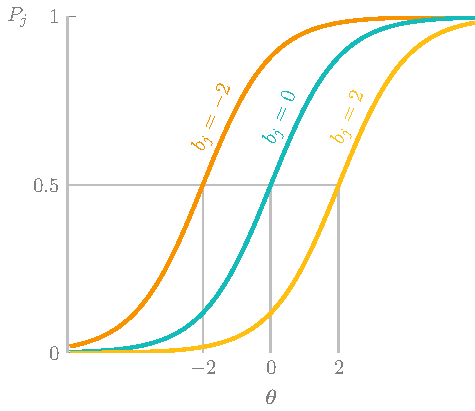
\includegraphics[page=1]{03-education/figures/tikzfigures.pdf}
    \caption[Item response functions of the 1PL model]{Three \glspl{irf} in the \gls{1pl} model, with different difficulty parameters $b_j$. The difficulty parameter represents the difficulty of the exercise. 
    For a fixed ability level, e.g. $\bm\theta = 0$, a higher difficulty means a lower probability $P_j$ of getting a correct answer.
    The probability of a correct answer is 50\% when $b_j = \bm\theta$.}
    \label{fig:1pl}
\end{figure}

There are more characteristics to an exercise than its difficulty. 
One characteristic that is useful to help estimate the ability of users is the discriminative ability of the exercise.
This characteristic represents how good an exercise is at differentiating between users of varying ability levels.
An extension to the \gls{1pl} model exists that includes this parameter, resulting in the \gls{2pl}. 
This second parameter $a_j$ of an item is a multiplicative parameter, as shown in the \gls{irf} in Equation~\ref{eq:2pl}.

\begin{equation}
    \label{eq:2pl}
    P_{j}(\bm{\theta}_i,\bm{p}_j) =
    Pr(X_{ij} = 1 | \bm{\theta}_i,a_j,b_j) =
    \frac{\exp\big[a_j(\theta_i - b_j)\big]}{1 + \exp\big[a_j(\theta_i - b_j)\big]}
\end{equation}

In Figure~\ref{fig:2pl} the \glspl{irf} are plotted for three exercises with the same difficulty $b_j = 0$ but various discriminative abilities. 
For all three \glspl{irf} the probability of a correct answer is still 0.5 for users with an ability level equal to the exercise difficulty.
However, the second parameter influences the steepness of the curve.
For larger discrimination parameters such as $a_3 = 4$, a smaller increase in ability $\bm\theta$ around the exercise difficulty level $b_j = 0$ leads to a more notable increase in probability of a correct answer $P_j$.
Such an exercise discriminates better between low and high ability users.
On the other hand, exercises with lower discrimination values, like $a_1 = 0.25$ result in flatter \glspl{irf} and do not allow as easily for such discrimination.

\begin{figure}
    \centering
    %\input{03-education/plots/2pl}
    \includegraphics[page=2]{03-education/figures/tikzfigures.pdf}
    \caption[Item response functions of the 2PL model]{Three \glspl{irf} in the \gls{2pl} model, with equal difficulty parameter $b_j$ but different discrimination parameters $a_j$. The discrimination parameter represents how well an exercise can differentiate between users of different ability levels $\bm\theta$. A higher value means a steeper increase in probability of a correct answer $P_j$ around the difficulty level $\bm\theta = b_j$.}
    \label{fig:2pl}
\end{figure}

%Figure~\ref{fig:its-architecture} shows the completed architecture of the \gls{its}, obtained by replacing the algorithmic components with the techniques explained in this section.
%
%\begin{figure}
%    \centering
%    \input{03-education/plots/its-filled}
%  \caption{todo}
%  \label{fig:its-architecture} 
%\end{figure}

\subsubsection{Model calibration}
Both the \gls{1pl} and \gls{2pl} models hold parameters of two types: item parameters $\bm{p}_j$ and person parameters $\bm{\theta}_i$. 
With enough data, both sets of parameters can be accurately estimated.
First, the item parameters are estimated independently of the ability levels, this is called the \textit{model calibration}. 
Next, the ability levels are estimated while keeping the item parameters fixed.

\Gls{irt} offers several model calibration techniques, mostly designed for item banks with several dozens of items.
The larger size of the item bank of \gls{scw} will cause longer execution times and more difficult convergence to stable estimates.
I solve this problem by splitting the item bank to several smaller item banks, for example one for each framework on the platform.
The resulting consequences are discussed in Chapter~\ref{ch:its-experiments}.

The calibration of the model consists of tuning the model parameters to maximize the likelihood of the observed data.
More formally, model calibration is maximizing the likelihood of the model $L(\bm\theta,\bm{p})$ with respect to all item parameters $\bm{p} = (\bm{p}_1,\dots,\bm{p}_J)$.
Because this likelihood is also dependent on all person parameters $\bm\theta = (\theta_1,\dots,\theta_I)$, direct maximization is not possible.
There are several possible techniques that can be used to overcome this.
The most well-known are \gls{jml}, \gls{cml}, and \gls{mml}~\cite{magis2017computerized}.

The \gls{jml} algorithm iteratively maximizes the full likelihood with respect to both person and item parameters until convergence is reached.

\Gls{cml} relies on properties specific to the Rasch model to replace unknown ability levels with known sufficient statistics which then allows for the estimation of the item parameters without requiring the estimation of the person parameters.

\Gls{mml} is formulated under the assumption that the ability is a random parameter.
In contrast to the \gls{cml}, it can be used for other \gls{irt} models besides the Rasch model~\cite{bartolucci2010point}.
It does not replace the person parameters by sufficient statistics, but aims to integrate out the person parameters from the maximization process~\cite{bartolucci2010point,magis2017computerized}.
A prior distribution for the ability parameters $f(\bm{\theta})$ is used to compute the marginal likelihood (or the expectation) of a response pattern as shown in Equation~\ref{eq:integrate-out}.

\begin{equation}
    \label{eq:integrate-out}
    P_{j}(\bm{p}_j) = \int_{\mathbb{R}} P_{j}(\bm{\theta}_i,\bm{p}_j) f(\bm{\theta}_i) d\bm{\theta}_i
\end{equation}

The prior distributions are often chosen as normal distributions.
The item parameters can then be estimated by maximizing the full likelihood, calculated as the product of all marginal pattern likelihoods.
Computing these marginal response pattern distributions was conceptually complex until efficient \gls{em} algorithms were implemented~\cite{magis2017computerized}.

In this work, I used the \gls{mml} approach as it has many advantages, such as its applicability to many types of \gls{irt} models, its ability to compare the fit of different models, and its ability to handle perfect response patterns (all correct or all incorrect answers).

\subsubsection{Ability estimation}
Once the item parameters are calibrated, they are set as fixed.
Estimating the person parameters is done through maximizing the \textit{likelihood function} shown in Equation~\ref{eq:wle1}, with respect to $\theta$. 

\begin{equation}
    \label{eq:wle1}
    L(\theta) = \prod_{j=1}^{J} \prod_{k=0}^{K_j} P_{jk}(\theta, \bm{p}_j)^{Y_{jk}}
\end{equation}

In this equation, $Y_{jk}$ equals one if the response category $k$ was chosen for item $j$ and zero otherwise.

Note that since the item parameters $\bm{p}_j$ are already calibrated and now set as fixed, the function only depends on the person parameters $\theta$.
Maximizing this function is equivalent to maximizing its logarithm, the so-called \textit{log-likelihood function}, as shown in Equation~\ref{eq:wle2}.

\begin{equation}
    \label{eq:wle2}
    l(\theta) = \sum_{j=1}^{J} \sum_{k=0}^{K_j} Y_{jk}\log P_{jk}(\theta, \bm{p}_j)
\end{equation}

For dichotomous items ($k \in \{0,1\}$), such as in our case, this can be written as:

\begin{equation}
    \label{eq:wle3}
    l(\theta) = \sum_{j=1}^{J} Y_{j1} \log P_{j}(\theta, \bm{p}_j) + Y_{j0} \log Q_{j}(\theta, \bm{p}_j)
\end{equation}

%\todo[inline]{I think this would be too much of a tangent on the actual work}
There are several calibration methods to maximize this likelihood, describing them is out of the scope of this book. 
The method applied in this work is the \gls{wle}~\cite{magis2017computerized}.

\subsection{Alternative approaches}
\gls{irt} is often used to adapt the learning material to the ability level of the student in e-learning systems~\cite{chen2005personalized,yarandi2011personalised}.
Often the \gls{irt} ability level is used to determine the appropriate difficulty level of the exercises that should be presented to the user~\cite{chen2005personalized,yarandi2011personalised,khanal2020systematic}.
In another approach the \gls{irt} ability level was used as a weight in \gls{cf} algorithms so that that the users with greater ability level have greater weight in the calculation of the recommendations than the users with less knowledge.
This approach assumes that users of greater ability level, such as teachers, are more able to assess the utility of an item than users of lower ability level.
In this work, however, users do not rate the items explicitly but instead the utility is determined from learning outcome and engagement, as will be explained in Section~\ref{sec:utility}.

Despite the popularity of \gls{irt} some alternative approaches exist to determine the ability level of a user.

\subsubsection{Classical Test Theory}
In \gls{ctt}, all users have to complete the same exercises and their accuracy on the questions is used as an indicator for the ability level.
Classic test theory assumes that each person has an unobservable true ability score $T$ that would be the result of a test if there are no errors in the measurement.
In a test, the observed score $X$ is measured instead.
This score is defined as the sum of the true score and a measurement error $E$.
According to \gls{ctt}, the true score is impossible to obtain, but several techniques exist to estimate the reliability of a test.

Besides the lower accuracy of ability estimation, \gls{ctt} is also not appropriate to use in the \gls{its} because it requires fixed item selection for all the users.
By doing this, some users are guaranteed to feel bored or frustrated since it is impossible to select items of the appropriate difficulty level for all of the users simultaneously.

\subsubsection{Other IRT models}
\paragraph{Three- and four-parameter logistic models}
In this work we are using the \gls{2pl} Rasch model of \gls{irt}.
However, further extensions exist on the \gls{2pl} model that add additional parameters.
The \gls{3pl} and \gls{4pl} add parameters that influence the lower and upper asymptotic behaviour of the \gls{irf}~\cite{magis2017computerized}.
The lower asymptote parameter $c_j$ is sometimes called the pseudo-guessing parameter. 
It allows the probability of a correct answer for infinitely small ability levels to be a positive probability instead of zero in the \gls{1pl} and \gls{2pl} model. 
Even users of extremely low ability level still have a non-zero probability of answering the exercise correctly.
In reality, this can of course be achieved through guessing the correct answer in case of multiple-choice.

On the opposite side of the curve, the upper asymptote parameter $d_j$ allows the maximal probability to be lower than one. 
This parameter is called the inattention parameter. 
The \gls{4pl} model allows users of extremely high ability level to have a probability of less than 1 of answering the exercise correctly.
This can be explained as the user being inattentive or hurried when answering the question.

The resulting \glspl{irf} are shown in Equations~\ref{eq:3pl} and \ref{eq:4pl}.
\begin{equation}
\begin{split}
    \label{eq:3pl}
    P_{j}(\bm{\theta}_i,\bm{p}_j)
    & = Pr(X_{ij} = 1 | \bm{\theta}_i,a_j,b_j,c_j) \\
    & = c_j + (1-c_j) \frac{\exp\big[a_j(\theta_i - b_j)\big]}{1 + \exp\big[a_j(\theta_i - b_j)\big]}
\end{split}
\end{equation}
\begin{equation}
\begin{split}
    \label{eq:4pl}
    P_{j}(\bm{\theta}_i,\bm{p}_j) =
    & = Pr(X_{ij} = 1 | \bm{\theta}_i,a_j,b_j,c_j,d_j)\\
    & = c_j + (d_j-c_j) \frac{\exp\big[a_j(\theta_i - b_j)\big]}{1 + \exp\big[a_j(\theta_i - b_j)\big]}
\end{split}
\end{equation}

\Glspl{irf} of the \gls{3pl} model with varying pseudo-guessing parameters are plotted in Figure~\ref{fig:3pl}.
In Figure~\ref{fig:4pl}, three \glspl{irf} are plotted with varying values for the inattention parameter.
The addition of these parameters is likely to improve the fit of the model to the data.
However, the pseudo-guessing and inattention parameters of exercises are not of much use in the \gls{its} or the \gls{scw} portal in general, and hence the \gls{2pl} model is chosen.

\begin{figure}
    \centering
    %\input{03-education/plots/3pl}
    \includegraphics[page=4]{03-education/figures/tikzfigures.pdf}
    \caption[Item response functions of the 3PL model]{Three \glspl{irf} in the \gls{3pl} model, with equal difficulty and discrimination parameters but different pseudo-guessing parameters $c_j$. The pseudo-guessing parameter represents the probability that a user is able to guess the correct answer to a question. A non-zero pseudo-guessing parameter means a non-zero probability of a correct answer $P_j$, even for users of extremely low ability level $\bm\theta$.}
    \label{fig:3pl}
\end{figure}

\begin{figure}
    \centering
    %\input{03-education/plots/4pl}
    \includegraphics[page=5]{03-education/figures/tikzfigures.pdf}
    \caption[Item response functions of the 4PL model]{Three \glspl{irf} in the \gls{4pl} model, with equal difficulty, discrimination, and pseudo-guessing parameters but different inattention parameters $d_j$. The inattention parameter represents the probability that a user answers incorrectly due to inattention. A inattention parameter different form 1 means that the probability of a correct answer $P_j$ is never 1, not even for users of extremely high ability level $\bm\theta$.}
    \label{fig:4pl}
\end{figure}

\paragraph{Polytomous IRT models}
%Predict WHICH of the answers is given (in multiple choice). For that it is necessary to know which one is MOST correct. Unfortunately this information is not available.
% The selection of a particular polytomous model involves a number of factors: the type of data, model-
%data fit, philosophical considerations, model assumptions, and parsimony. If the data consist of items that have unordered alternatives, then the NRM is appropriate. When responses to an item are classified into more thantwo categoriesthatcan beorderedtorepresentvaryingdegreesofthetraitmeasuredbytheitem, theneithertheGRM,GPCM,orthePCMcouldbeused.Iftheordereddataareratings,thenmoreconstrained versionsofthesemodels,suchastheMRSM,theSIM,ortheARSM,wouldbeappropriate.~\cite{dodd1995computerized}
In the \gls{2pl} model, we are only concerned with whether or not the selected answer is correct.
However, even if an incorrect options is selected, it is often possible to use this information to refine the estimate of the ability level of the user based on which incorrect option was chosen~\cite{magis2017computerized}.
This is the intent of polytomous \gls{irt} models.
There are many polytomous models available but they generally require scoring in a way that partial credit can be given for incorrect answers~\cite{dodd1995computerized}.
This makes sense if one considers scoring essays based on quality, or giving partial credit in mathematical questions for completing some of the steps.

On the \gls{scw} portal this could be achieved by ranking the options in the multiple choice question from the most incorrect to the most correct.
However, currently this is not the case, so we have no indication of which incorrect answer is closest to correct.
Furthermore, historically the incorrect answers have not been logged in the data collection, only the amount of incorrect guesses before a correct answer is given.
In case the user gave up before finding the correct answer (or in assessments where only one guess is available), the last guess is logged.
Polytomous models could result in more accurate results, however, currently they can not be used to the available data set.

\paragraph{Multidimensional IRT models}
While the ability level has been introduced as a multivariate vector of latent traits $\bm{\theta}_i$, in Section~\ref{sec:irt-intro}, in the current implementation this has been implemented as a scalar.
In reality, the ability of a user regarding software security is not accurately represented as a single value.
When the ability estimate is represented as a vector, a value can be obtained for each dimensions of the skill.
For example, the ability of a user for each of the vulnerability categories can be represented as a scalar.
Using a multidimensional representation for the ability level like this, is not only likely to result in more accurate estimates, but also allows more granular decision making of the appropriate difficulty for an item in the \gls{its}.
However, sufficient data needs to be available to have an accurate measurement for each of the dimensions which would limit the amount of users that can be accurately assessed.
I have opted to keep as much data as possible to train the \gls{cf} algorithm instead.

\paragraph{Response-time IRT models}
Response-time \gls{irt} models also take into account how much time each user takes to answer a correct answer.
However, as mentioned before, there have been several bugs present in the time tracking features on the platform and this data is currently unreliable.

Furthermore, time pressure varies in different modes on the platform.
While users can generally take as much time as they prefer when answering questions in training and assessments, in tournaments there is a limited time to complete the questions.

\subsubsection{Elo system}
The Elo rating system is a method for calculating relative skill levels between players of a zero-sum game~\cite{elo1978rating}.
It is named after its inventor Arpad Elo.
The system is widely used in sports, games, and videogames, such as chess, American football, basketball, Major League Baseball, table tennis, Scrabble, Counter Strike: Global Offensive, and League of Legends.

Similarly to \gls{irt}, the ability level is not measured directly, but it is inferred from wins, losses, and draws against other players or teams.
Based on the current ability levels, the expected outcome of a match-up is predicted.
When the actual outcome differs from this expectation, the ability level is updated~\cite{elo2008logistic}.
By how much it is updated depends on the difference between the ability levels, and in some cases by the observed skill difference.
For an overwhelming victory a bigger increase in ability will often be awarded than for a near win.

The Elo system is designed for symmetric match-ups such as player versus player, or team versus team.
A zero-sum game is a mathematical representation of a situation in which an advantage that is won by one player is lost by the other.
While \gls{irt} sets both users and items on the same scale, the training platform can not be considered a zero-sum game.
One challenge is played by many more players than a single player usually plays challenges.

Although adaptations exist for asymmetric games~\cite{wise2021elo}, I expect the ability estimates to converge slower and the difficulty estimates of items to be less stable than with \gls{irt}.
\Gls{irt} takes into account the entire response pattern, hence it is able to estimate the outcome of a challenge again later, based on new information.
The Elo system only takes into account the current ability of the user, which might still be inaccurate at the time of playing.
As a result, potentially large updates are made to the difficulty of the items that are presented to this user.